\chapter{Grundlagen}
\label{chapter:grundlagen}

In diesem Kapitel werden die für diese Arbeit relevanten theoretischen und konzeptuellen Grundlagen beschrieben. Begonnen wird mit einer kurzen Einführung in das Brettspiel Patchwork. Anschließend widmet sich dieses Kapitel der Spieltheorie, einem mathematischen Bereich, der bei der Modellierung und Analyse von Entscheidungssituation verwendet wird. Dann wird der Minimax-Algorithmus betrachtet, der den grundlegenden Algorithmus für einen in dieser Arbeit implementierten Computergegner darstellt. Anschließend werden die Grundlagen für zwei weitere Computergegner geschaffen, indem die Theorie von \acl{MCTS} und AlphaZero erläutert wird. Abschließend werden interaktive System erläutert, die für die Gestaltung der Benutzerschnittstellen und Spielererfahrung der Computerumsetzung des Brettspiels wichtig sind.

\section{Brettspiel Patchwork}
\label{chapter:brettspiel-patchwork}

\begin{wrapfigure}{r}{0.325\textwidth}
    \centering
    \vspace*{-0.75cm}
    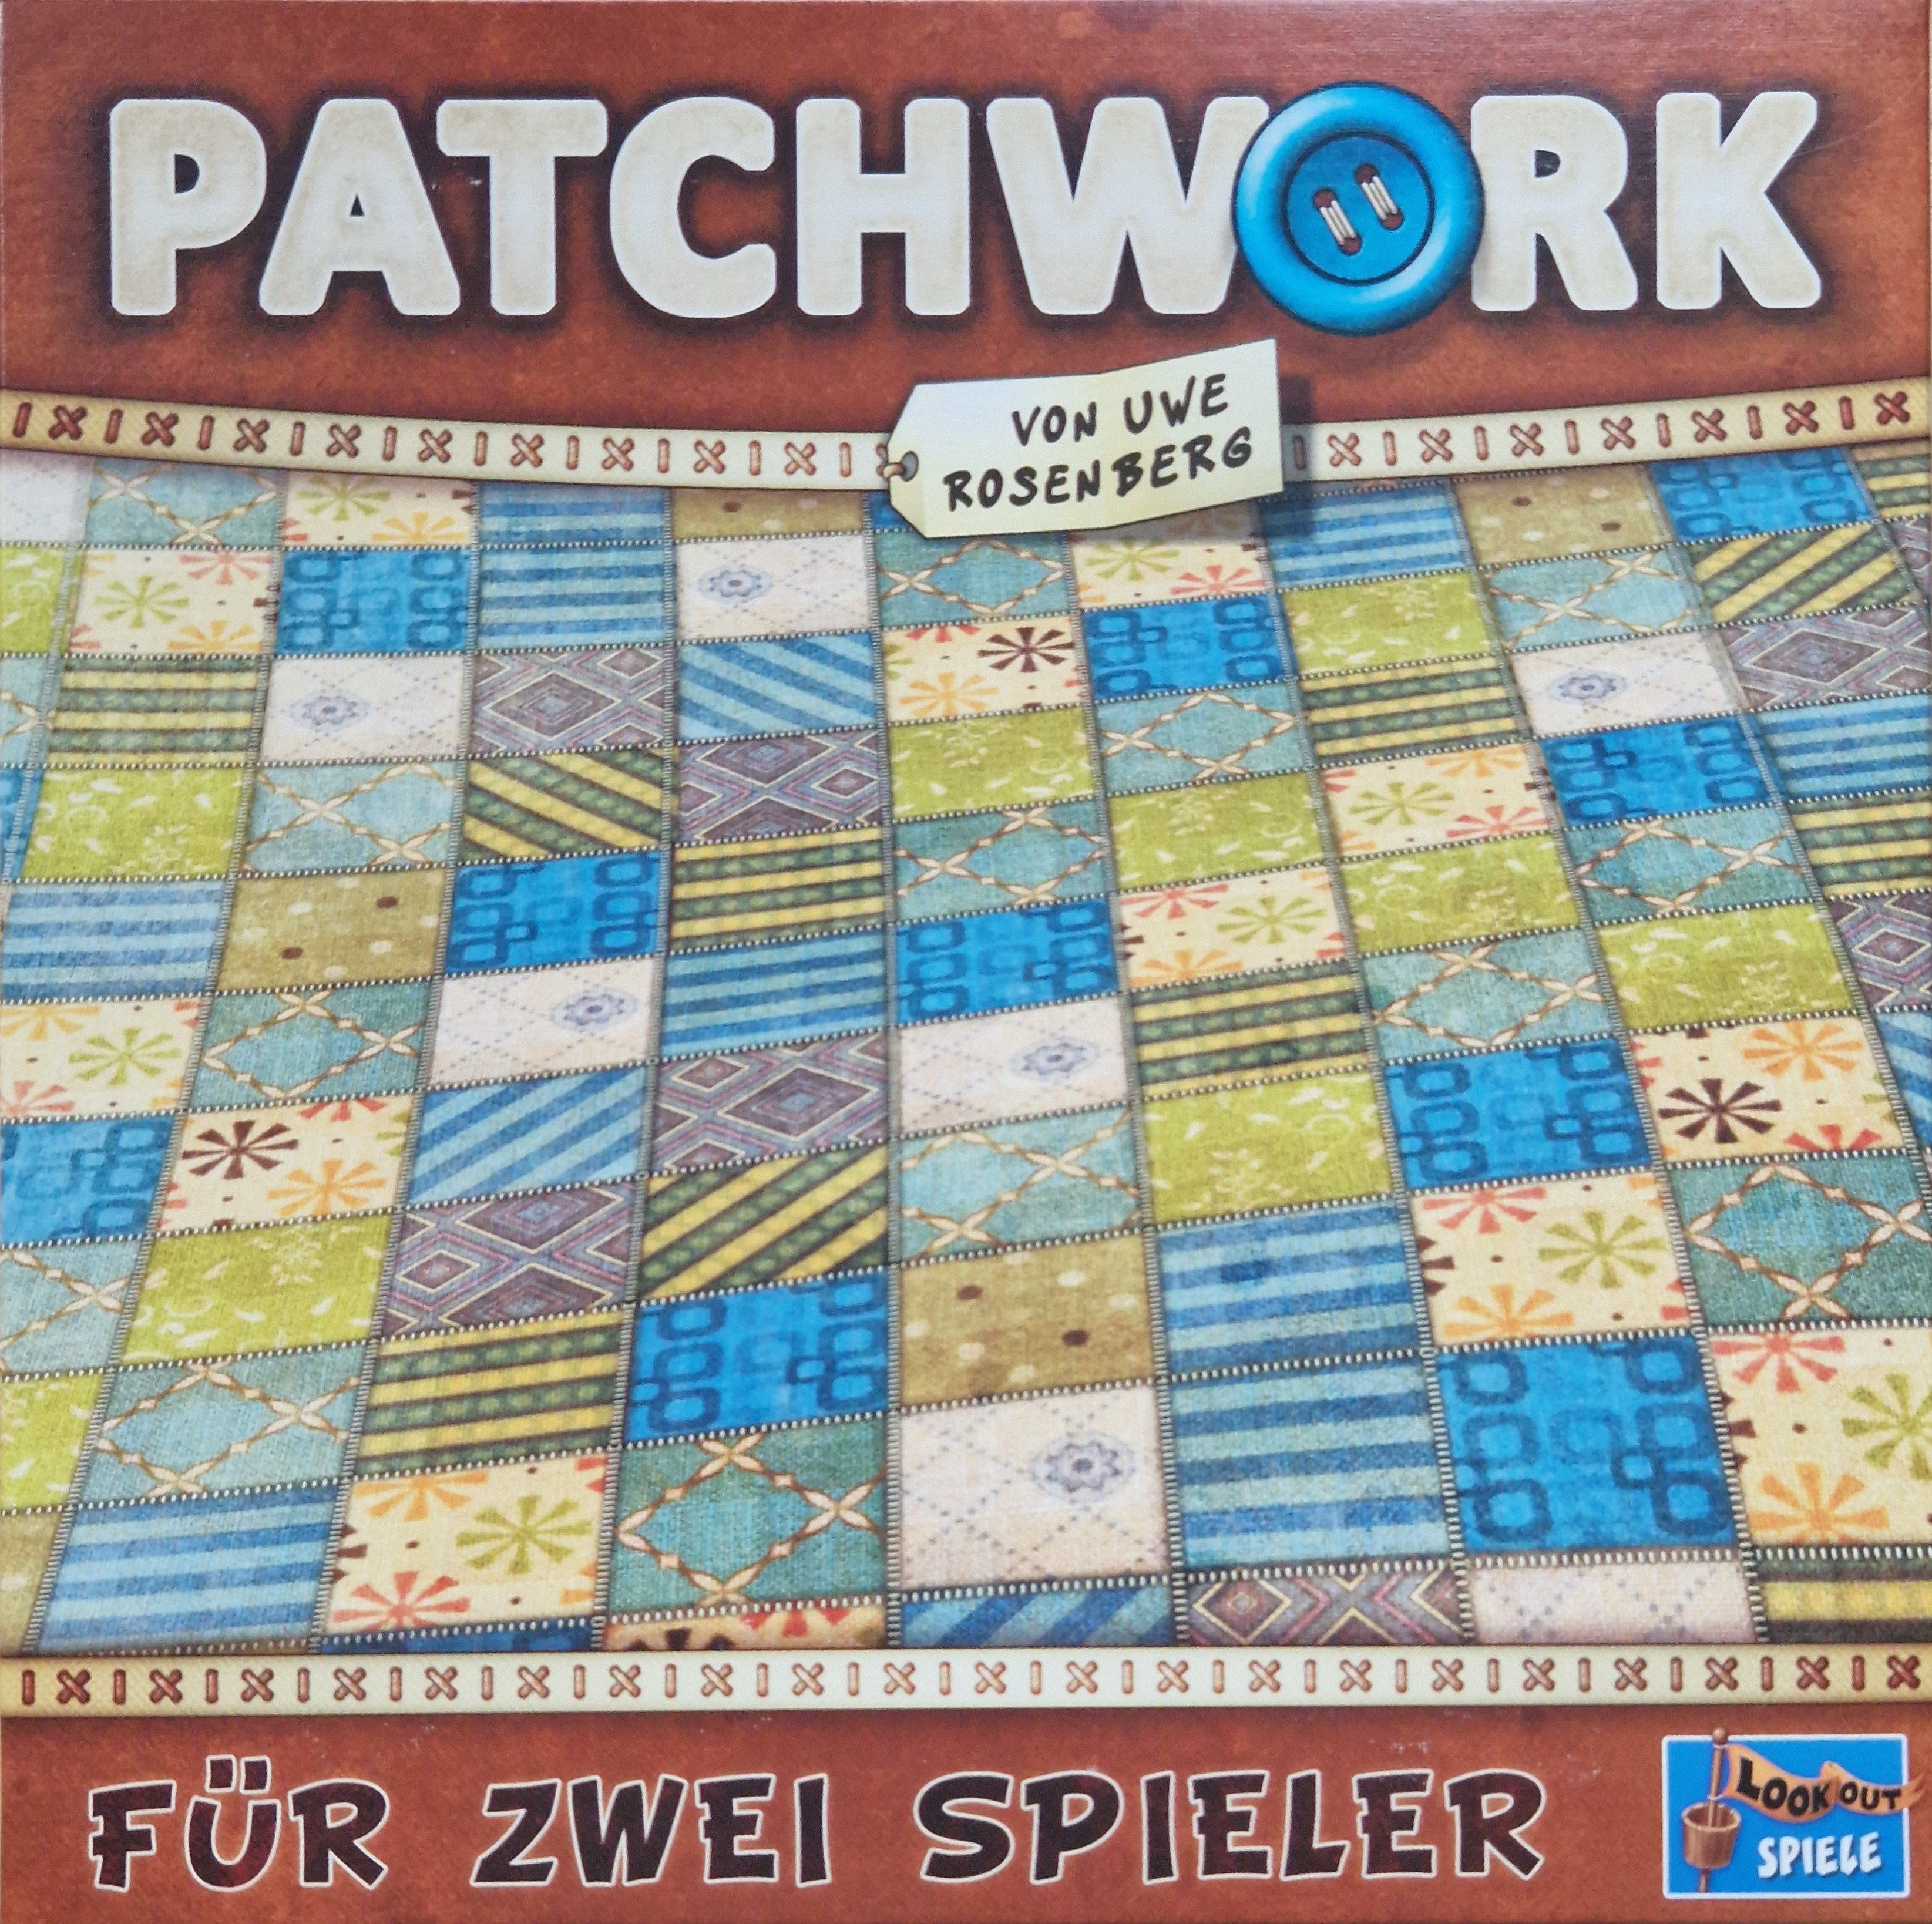
\includegraphics[width=0.28\textwidth]{res/pictures/assets/patchwork-cover.png}
    \caption[Cover von Patchwork]{\unskip}
    Cover von Patchwork
    \label{fig:patchwork-cover}
    \vspace*{-0.75cm}
\end{wrapfigure}

Patchwork ist ein Brettspiel von Uwe Rosenberg, das 2014 bei Lookout Spiele erschienen ist. Bei dem Brettspiel spielen zwei Spieler vom Alter 8 Jahre und aufwärts gegeneinander, wobei ein Spiel in der Regel ungefähr 30 Minuten lang ist \cite{LookoutSpielePatchwork}. Bei dem Brettspiel gestalten zwei Spieler jeweils eine eigne Decke aus Stoffresten, Flicken und Knöpfen, der Technik entsprechend, die der Titel vorgibt. \cite{SpielDesJahresPatchwork}

Das Ziel der Spieler ist mit den gegebenen Stoffplättchen unterschiedlicher Formen und Größen die vorgegebene Fläche zu füllen. Das Puzzlespiel erfordert taktisches Gespür, da die Flickenauswahl die Zugfolge und auch die Flickenauswahl des Gegenspielers beeinflusst. Immer können die Spieler jedoch nicht die gewünschten Flicken verwenden, da diese mit der Spielwährung Knöpfe aus der eigenen Kasse bezahlt werden müssen. An die begehrten Knöpfe kommen die Spieler über die bereits eingearbeiteten Flicken, welche Knöpfe auf sich abgebildet haben. Je mehr dieser Knöpfe auf der eigenen Decke abgebildet sind, desto höher das Einkommen an Knöpfen. Wer am Schluss des Spiels die meisten Knöpfe erwirtschaftet und seine Decke gut bestickt hat, gewinnt den Nähwettstreit. \cite{SpielDesJahresPatchwork}

\section{Spieltheorie}
\label{chapter:spieltheorie}

TODO:

\subsection{Spielbaum}

TODO: Spielbaum, Entscheidungsbaum

\subsection{Spielkomplexität}

TODO:

\begin{itemize}
    \item \textbf{Zustandsraum-Komplexität}: TODO:
    \item \textbf{Spielbaumgröße}: TODO:
    \item \textbf{Entscheidungskomplexität}: TODO: needed?
    \item \textbf{Spielbaumkomplexität}: TODO:
\end{itemize}

\section{Minimax-Algorithmus}
\label{chapter:minimax-algorithmus}

TODO:

Hier haben wir mehr

\section{Monte Carlo Tree Search}
\label{chapter:monte-carlo-tree-search}

\acf{MCTS} ist ein Suchalgorithmus, welcher verwendet wird, um in einem Spiel die beste Aktion zu finden. Dazu wird der Algorithmus während der Entscheidungszeit des Computerspielers ausgeführt. Innerhalb dieser Zeit wird schrittweise ein Suchbaum erstellt. Dabei wird für jede Aktion eine Heuristik erstellt, indem sehr viele Spiele zufällig bis zum Ende ausgespielt werden. Dadurch ergibt sich über die Zeit eine Wahrscheinlichkeit für das Ergebnis des Spiels für jede mögliche Aktion \cite[S. 61]{2008.ParallelMCTS}. Der \ac{MCTS}-Suchprozess besteht aus vier Phasen:

\begin{enumerate}
    \item \textbf{Selektion}: Der Suchbaum wird beginnend ab dem Wurzelknoten bis zu einem Blattknoten durchlaufen, indem in jeder Ebene immer genau ein Kindknoten nach einer bestimmten Richtlinie ausgewählt wird. \cite[S. 187]{2018.ReinforcementLearning}
    \item \textbf{Expansion}: Der ausgewählte Blattknoten wird um ein weiteres Kind erweitert, indem ein noch nicht erforschte Aktion ausgeführt wird. \cite[S. 61]{2008.ParallelMCTS}
    \item \textbf{Simulation}: Ausgehend vom neu hinzugefügten Knoten wird das Spiel bis zum Ende simuliert, indem bis Spielende zufällige Aktionen ausgeführt werden. \cite[S. 61]{2008.ParallelMCTS}
    \item \textbf{Backpropagation}: Das Ergebnis der Simulation wird durch den Suchbaum rückpropagiert, indem das Ergebnis (Gewonnen oder Verloren) ausgehend von dem in Zweitens neu hinzugefügten Knoten bis zum Wurzelknoten hochgereicht wird. \cite[S. 187]{2018.ReinforcementLearning}
\end{enumerate}

Die vier Phasen sind anschaulich in Abbildung \ref{fig:mcts-phases} dargestellt. Diese Phasen werden so lange wiederholt, bis die Entscheidungszeit vorbei ist.

\begin{figure}[!ht]
    \centering
    
\includegraphics[width=\textwidth]{res/pictures/mcts-phases.pdf}
    \caption{Phasen des \acs{MCTS} Algorithmus}
    \label{fig:mcts-phases}
\end{figure}

Für die erste Phase der Selektion wird im Normalfall die in \ref{eqn:uct} dargestellte \ac{UCT} Formel verwendet. Die \ac{UCT} Formel balanciert die Entscheidung zwischen der Ausnutzung von bereits bekannten Aktionen mit der Erkundung von unsicheren Aktionen \cite[S. 206]{2009.ComputerGoMCTS}. Dazu wird im ersten Teil die Anzahl der Siege ($w$) durch die Anzahl der Besuche des Kindknotens ($n$) geteilt. Dieser Term wird immer größer, je öfters eine Simulation nach einem Knotenbesuch gewonnen wird. Der andere Term wird immer größer, je weniger ein Knoten im Vergleich zu seinem Elternknoten ($N$) besucht wird und erzwingt somit auch die Erkundung weniger besuchter Knoten. Bei $c$ handelt es sich um eine Erkundungskonstante, welche das Verhältnis zwischen Ausnutzung und Exploration regelt und normalerweise auf $\sqrt{2}$ gesetzt wird.

\begin{equation}
    \label{eqn:uct}
    \mathbb{U}\mathbb{C}\mathbb{T} = \frac{w}{n} + c \cdot \sqrt{\frac{\ln N}{n}}
\end{equation}

Ein entscheidender Vorteil von \ac{MCTS} ist, dass keine statische Evaluierungsfunktion einer Position wie bei vergleichbaren Algorithmen existieren muss \cite[S. 61]{2008.ParallelMCTS}, da durch zufällige Erkundungen eines Teils des Suchbaums eine Approximation für den tatsächlichen Wert geschaffen wird. \ac{MCTS} hat sich vor allem für Spiele mit einer sehr großen Anzahl an Aktionen bzw. möglichen Zuständen als besser geeignet als traditionelle \hyperref[chapter:minimax-algorithmus]{Minimax}-basierte Programme herausgestellt \cite[S. 1]{2013.MCTSAndMinimaxHybrids} und ist aus diesem Grund auch zu großen Teilen für die Verbesserung der Computergegner in solchen Spielen wie beispielsweise Go verantwortlich \cite[S. 2006]{2009.ComputerGoMCTS} \cite[S. 185]{2018.ReinforcementLearning}.

\section{AlphaZero}
\label{chapter:alphazero}

TODO:

\section{Interaktive Systeme}
\label{chapter:interaktive-systeme}

TODO:

